\documentclass{article}
\usepackage{amsfonts}          % Para las negrita de pizarra
\usepackage{indentfirst}       % Para que quede mas lindo el formateo
\usepackage{graphicx}          % Para graficos
\usepackage{minted}            % Para poner codigo y que quede con sintaxis fachera
\usepackage{hyperref}          % Para meter hipervinculos
\usepackage[dvipsnames]{xcolor}% Para usar colores
\usepackage{hhline}            % Mas configuracion para las líneas en tablas
\usepackage{amsmath}           % Agregado para tags de ecuaciones
\usepackage{xcolor}            % Coloreado de ecuaciones
\usepackage{quoting, xparse}   % Usado para citar
% \usepackage{svg}               % Para usar imagenes svg que se ven lindas independientemente del zoom. WARNING REQUIERE DE INKSCAPE. Tal vez no vale la pena
\usepackage{amsmath}

\graphicspath{ {./images/} }

\newcommand{\docuPy}{%
  {\href{https://wiki.python.org/moin/TimeComplexity}{documentacion oficial}}
  }%

  % Comandos para facilitar el citado
  % Fuente: https://tex.stackexchange.com/a/391739/273865
\NewDocumentCommand{\bywhom}{m}{% the Bourbaki trick
  {\nobreak\hfill\penalty50\hskip1em\null\nobreak
   \hfill\mbox{\normalfont(#1)}%
   \parfillskip=0pt \finalhyphendemerits=0 \par}%
}

% Esta funcion en realidad es una mentira. Emula ser una funcion de latex. La idea
% es que el makefile que corre esto vea la funcion y la reemplace correctamente
% 
\newcommand{\funcionArchivo}[2]{%
  {\textcolor{red}{WARNING: SI ESTAS VIENDO EN EL PDF SIGNIFICA QUE ALGO ANDUVO MAL. ASEGURATE DE COMPILAR EL LATEX CON EL MAKEFILE. GRACIAS :D}}
  }%

\begin{document}

\begin{titlepage}
  \vspace*{1cm}

  \begin{center}
    {\Huge{Trabajo Práctico 2: Programación Dinámica para el Reino de la Tierra}}
  \end{center}

  \vspace{0.4cm}

  \begin{center}
    {\LARGE{Facultad de Ingeniería de la Universidad de Buenos Aires}}\\
    \vspace{0.3cm}
    {\Large{Teoría de Algoritmos}}\\
    \vspace{0.3cm}
    {\large{Cátedra Buchwald-Genender}}\\
  \end{center}

  \vspace{0.8cm}
  \begin{center}
    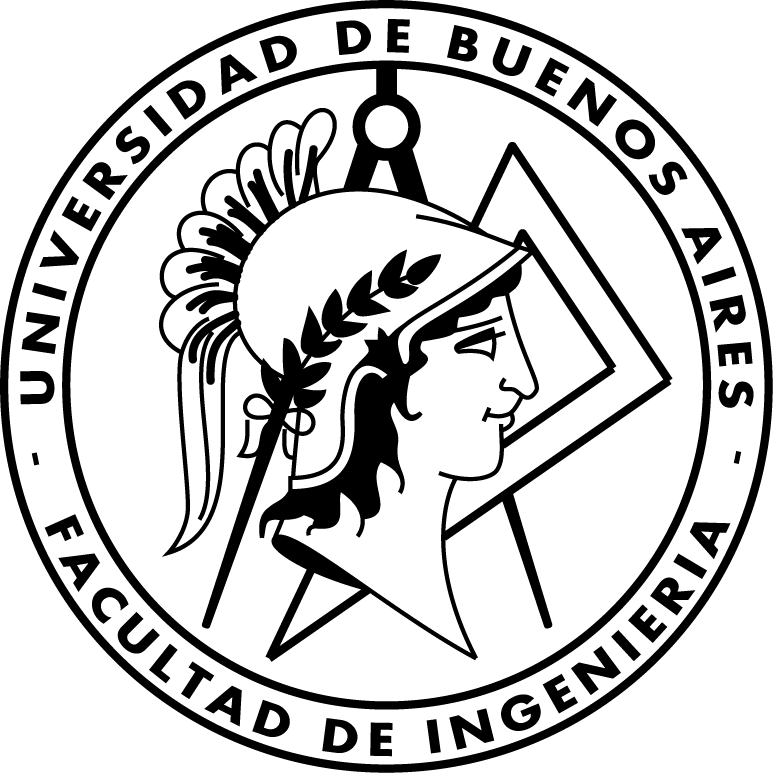
\includegraphics[scale=0.8]{Logo-fiuba}
  \end{center}

  \vspace{1.4cm}
  \begin{center}

    {\begin{minipage}[t]{.32\textwidth}
        \begin{center}
          Gómez Belis, Sofía\\
          {\small{Padrón: 109358}}\\
          {\small{email: sgomezb@fi.uba.ar}}
        \end{center}
          \end{minipage}
          \begin{minipage}[t]{.32\textwidth}
        \begin{center}
          Llanos Pontaut, Valentina\\
          {\small{Padrón: 104413}}\\
          {\small{email: vllanos@fi.uba.ar}}\\
        \end{center}
      \end{minipage}
      \begin{minipage}[t]{.32\textwidth}
        \begin{center}
          Orsi, Tomas Fabrizio\\
          {\small{Padrón: 109735}}\\
          {\small{email: torsi@fi.uba.ar}}
        \end{center}
      \end{minipage}}

  \end{center}
\end{titlepage}

\renewcommand*\contentsname{Indice}
\tableofcontents
\pagebreak

\section{Análisis del problema}
\subsection{Descripción y objetivo}

El objetivo de este trabajo práctico es implementar un algoritmo de programación dinámica para ayudar a los Dai Li, la policía secreta de la ciudad Ba Sing Se del Reino de la Tierra, en su combate contra la Nación del Fuego. Como somos sus jefes estratégicos, debemos reportarles las estrategias que deberían emplear en cada minuto del ataque con el fin de eliminar la máxima cantidad de maestros Fuego.

Afortunadamente, las mediciones sísmicas de los Dai Li nos permitieron obtener información de la cantidad de enemigos que llegan en cada minuto. Además, sabemos que la cantidad de enemigos no es acumulativa; después de cada ataque, los enemigos se retiran. Tenemos entonces, una lista de valores $x_i$ que ilustran este hallazgo. Por otro lado, la potencia de los ataques de fisura de la policía secreta dependen de cuánto tiempo fue cargada la energía. La función monótona creciente $f(\cdot)$ indica que, si transcurrieron $j$ minutos desde que se utilizó este ataque, entonces se podrá eliminar hasta  $f(j)$ soldados enemigos. Como este valor puede ser mayor a la cantidad de maestros Fuego, en el minuto $k$ se podrá eliminar $min(x_k, f(j))$ soldados, perdiendo además la energía acumulada. En el primer minuto, en caso de decidir atacar, les corresponde $f(1)$ de energía.

Sabiendo la duración en minutos del ataque ($n$), y los valores de $x_i$ y $f(j)$, podemos analizar el problema presentado e informarles a los Dai Li la secuencia de estrategias que les permitirá eliminar la mayor cantidad de enemigos empleando ataques de fisuras.

\subsection{Análisis y ecuación de recurrencia}

La resolución de un problema por medio de la programación dinámica implica reutilizar las soluciones a subproblemas más pequeños en subproblemas más grandes que los incluyan. En el contexto actual, el foco está puesto en maximizar la cantidad de enemigos eliminados dados $n$ minutos. Esta variable $n$ es crucial en el análisis del problema planteado puesto que si se tiene $k$ minutos, con $k < n$, necesariamente la cantidad de enemigos eliminados será menor o igual a la solución en el minuto $n$, siendo igual en el caso de que no lleguen más enemigos entre $k$ y $n$ minutos. De esta forma, la cantidad de minutos que tiene el ataque repercute en el resultado final del combate. Por ejemplo, si $n = 0$, se puede afirmar que la cantidad de enemigos eliminados será también 0. Entonces, nuestros subproblemas estarán dados por la cantidad máxima de enemigos que se pueden eliminar en cada minuto $i \leq n$.

Sabiendo la forma de los subproblemas, debemos analizar cómo se componen para resolver subproblemas más grandes. Si queremos obtener la solución óptima en el minuto $i$, vamos a poder utilizar las soluciones parciales calculadas hasta entonces, pero no nos interesa si existen o no problemas más grandes. En cada minuto $i < n$ hay solamente dos estrategias posibles: atacar o cargar. \textbf{Atacar} implica enfrentarse con el enemigo, derrotando $f(j)$ soldados (con $j$ siendo la cantidad de minutos desde el ataque anterior) y perdiendo la energía acumulada. En cambio, definimos \textbf{cargar} como la acción de decidir no atacar y acumular más energía para un ataque futuro. 

Sin embargo, en el caso del minuto $i = n$, ¿tiene sentido cargar sabiendo que no van a llegar más enemigos en el futuro? No. Ésto se debe a que la cantidad de maestros Fuego que se podrá eliminar en ese minuto será mayor o igual a 0, pero si cargamos energía, será definitivamente nula. Por lo tanto, en el último minuto conviene siempre atacar. Ahora bien, como establecimos antes, en el minuto $i \leq n$ no importa si $i = n$ o $i < n$, solamente debemos calcular el óptimo actual. En base al análisis previamente presentado, siempre va a ser mejor atacar a cargar, más allá de que en la solución final (problema mayor) se lleve a cabo la estrategia opuesta debido a que eso esté contemplado en el óptimo del minuto $n$. 

Si en el minuto $i$ los Dai Li atacan, la cantidad de enemigos eliminados en ese instante será $min(f(j), x_i)$. El valor de $x_i$ es conocido, pero la energía acumulada ($f(j)$) por la policía secreta de la ciudad depende de los minutos que pasaron desde el último ataque. De esta manera, tenemos una segunda variable involucrada en el problema: $j$. Si el último ataque fue realizado hace un minuto, actualmente se podrá eliminar $min(f(1), x_i)$ soldados y la cantidad de enemigos eliminados acumulada será la suma entre este valor y el correspondiente en el ataque anterior. 

¿Qué sucede si el óptimo hace dos minutos es mayor que en el minuto anterior o su suma con $min(f(2), x_i)$ lo es? Como queremos maximizar el resultado final, claramente nos conviene haber atacado hace dos minutos, lo cual también indica que en el minuto $i - 1$ se cargó energía. Tenemos varias opciones para el ataque anterior, más precisamente $1 \leq j \leq i$, pero utilizaremos aquel que nos lleve a la mejor solución. Entonces, el óptimo para el minuto $i$ será la suma entre $min(f(j), x_i)$ y el óptimo en el minuto $i - j$.

Sabiendo la forma de los subproblemas y la manera en que éstos se combinan, podemos plantear la \textbf{ecuación de recurrencia} para el minuto $i$:

$$OPT[i] = max(min(f(j), x_i) + OPT[i - j] \forall j \in [1; i])$$

Como caso base, tenemos que en el minuto 0 se eliminan 0 enemigos.

Encontrada la ecuación de recurrencia, procedemos a aplicarla iterativamente de manera bottom up, construyendo las soluciones a los subproblemas de $i < n$ hasta llegar a la solución del problema original con $i = n$. Esta técnica es justamente programación dinámica. Empleamos \texttt{memoization} guardando los resultados calculados previamente en un arreglo. El procedimiento explicado nos permite realizar una exploración implícita del espacio de soluciones. La solución final será óptima porque en el minuto $n$ elegimos haber atacado hace $j$ minutos, donde $j$ maximiza la ecuación de recurrencia.

Como conclusión, el uso de esta ecuación de recurrencia en nuestra implementación nos permite determinar la cantidad máxima de enemigos que se pueden atacar. En cada minuto calculamos el  máximo número de adversarios eliminados si se decide atacar en ese instante. Este valor está determinado por el tiempo entre éste y el ataque anterior. Al quedarnos con un $j$ que maximice la suma final de enemigos derrotados en el minuto $i$, nos aseguramos de obtener una solución óptima a ese subproblema. Luego, en el último minuto del combate, utilizaremos las soluciones a estos subproblemas de forma tal que tendremos en cuenta el ataque anterior que ocurrió en el minuto $k = n - j$, donde $OPT[k] + min(f(j), x_n)$ maximiza la cantidad de enemigos eliminados en total. A su vez, el $OPT[k]$ tiene lo mismo en consideración. 

Guardar los óptimos en un arreglo de soluciones parciales para cada minuto nos facilita reconstruir la estrategia de ataque óptima que permite obtener el resultado para $OPT[n]$. Sabiendo el valor de la cantidad de enemigos que llegan en el minuto $n$, $x_n$, podemos comparar resultados parciales con $OPT[n]$ para obtener $j$. Es decir, como ya determinamos que en el minuto $n$ vamos a atacar, $j$ va a corresponder al resultado que cumpla con $OPT(n) = OPT(k) + min(f(j), x_n)$, siendo $k$ el minuto en que previamente se realizó un ataque ($k = n - j$). Entre $k$ y $n$, la estrategia empleada es recargar fuerzas.

Repetimos el procedimiento para $k$, hasta llegar al minuto 0. 

\section{Complejidad algorítmica}
\subsection{Complejidad lectura de archivos}
Antes de comenzar el algoritmo, tenemos que generar las listas de elementos sobre las cuales éste va a operar.
Para esto tenemos la siguiente porción de código:
\funcionArchivo{codigo/archivos.py generarTestDe}

La función lee la línea que contiene la cantidad de valores que van a tener ambas listas. Una vez hecho eso, lee $n$ líneas para almacenar los distintos valores de $x_i$ y luego lee otras $n$ líneas para tener los valores de $f(j)$. Esto tiene una complejidad temporal $O(2\cdot n)$ que, despreciando la constante, resulta $O(n)$.

\subsection{Complejidad algoritmo}
\funcionArchivo{codigo/algoritmo.py eliminar_enemigos}
El algoritmo empieza creando una lista de tamaño $n + 1$. Según la \docuPy, esto conlleva $\mathcal{O}(n)$ ya que se realiza $n$ veces una operación de tiempo constante $\mathcal{O}(1)$.

Luego, en la línea \texttt{7} comienza un ciclo \texttt{for} que recorre todos los valores de $n$. En la línea \texttt{9} comienza un nuevo ciclo \texttt{for}, el cual va desde 0 hasta el minuto actual $i$. Esto significa que, en el peor de los casos, este ciclo va a iterar hasta $n$. Dentro del ciclo, todas las operaciones son $\mathcal{O}(1)$, es decir, constantes.

Al tener dos ciclos anidados que realiza la cantidad de iteraciones mencionadas, podemos afirmar que la complejidad algorítmica de las líneas \texttt{7} a \texttt{17} es $\mathcal{O}(n^2)$.

Luego, en la línea \texttt{20} se ejecuta la función \texttt{obtener\_secuencia\_estrategias}, la cual analizamos en \nameref{sec:reconstruccion}. Sin embargo, podemos adelantar que su complejidad será también cuadrática.

Finalmente, en la línea \texttt{21} se ejecuta el método \texttt{reverse()}, el cual tiene complejidad $\mathcal{O}(n)$

Es decir, que el algoritmo de programación dinámica tiene una complejidad 
$$
\mathcal{T}(n) = 2 \cdot \mathcal{O}(n^2) + \mathcal{O}(n) = \mathcal{O}(n^2)
$$


\subsection{Complejidad reconstrucción de la solución}
\label{sec:reconstruccion}

\funcionArchivo{codigo/algoritmo.py obtener_secuencia_estrategias}
La reconstrucción de la secuencia estratégica empieza desde el último minuto, hasta 0.
Vemos que en la línea \texttt{26} tenemos un ciclo \texttt{while}, el cual tiene dentro un ciclo \texttt{for}.
Dentro del \texttt{for} todas las operaciones son de complejidad $\mathcal{O}(1)$.

En el peor de los casos, podemos pensar a estos dos ciclos como dos ciclos anidados que iteran desde 0 hasta $\texttt{n}$. Por esto, decimos que la reconstrucción va a tener una complejidad de $\mathcal{O}(n^2)$.

\subsection{Efecto de las variables sobre el algoritmo}
La complejidad obtenida es tenida en cuenta para el peor caso posible. Sin embargo, existe la posibilidad de que se ejecute en $O(n)$ si se recibe un set de datos con determinadas características.

Este es el caso cuando todos los datos de $x_i$ son menores al resultado de $f[0]$ que se corresponde con un minuto de diferencia con el ataque anterior, es decir, $f(1)$. Esto se debe a que el resultado será predecible ya que se podría derrotar al 100\% de enemigos en todos los ataques sin necesidad de cargar fuerzas.

La comprobación de si el conjunto de datos de entrada cumple esta condición es realizada antes de ejecutar el algoritmo propiamente dicho. Es decir, primero utilizamos la función \texttt{esOptimizable(n, x, f)} que hace la verificación en tiempo lineal. Si efectivamente cumple el requisito, \texttt{eliminar_enemigos_optimizado(n, x)} resuelve el problema planteado en tiempo $O(n)$ sumando la totalidad de enemigos y estableciendo una secuencia en la que siempre se ataca. Si bien este algoritmo no es de programación dinámica, creemos que es fundamental tenerlo en cuenta especialmente con sets de datos muy grandes donde la complejidad lineal por sobre la cuadrática puede hacer una gran diferencia en el timepo de ejecución.
Por el contrario, si no se puede optimizar, entonces ejecutamos nuestro algoritmo de programación dinámica. En este caso realizar la comprobación no afecta la complejidad resultante, sigue siendo $O(n^2)$.

\funcionArchivo{codigo/algoritmo.py esOptimizable}

\funcionArchivo{codigo/algoritmo.py eliminar_enemigos_optimizado}

\section{Ejemplos de ejecución}
Se pueden encontrar en la carpeta \texttt{ejemplos\_adicionales} del \href{https://github.com/La-sociedad-del-silencio/TP2-Dinamica}{repositorio entregado} algunos ejemplos de posibles ejecuciones creadas para corroborar la optimalidad del algoritmo planteado.

Además de los ejemplos brindados por la cátedra, se pensó en distintas perspectivas que podrían \textit{comprometer} de alguna manera la solución del algoritmo. Algunos aspectos evaluados fueron:

\begin{itemize}
    \item Momento en el que realiza el primer ataque:
    \begin{itemize}
        \item \texttt{atacar\_al\_inicio:} El primer ataque es al inicio del combate
        \item \texttt{atacar\_a\_la\_mitad:} El primer ataque es a la mitad del combate
        \item \texttt{atacar\_al\_final:} El primer ataque es al final del combate
        \item \texttt{atacar\_siempre:} No conviene nunca reservar energía, ataca siempre
    \end{itemize}
    \item Relación numérica entre $x_i$ y $f(j)$
        \begin{itemize}
        \item \texttt{x\_menor\_a\_f:} Todos los $x_i$ son menores a todos los $f(j)$
        \item \texttt{x\_mayor\_a\_f:} Todos los $x_i$ son mayores a todos los $f(j)$
        \item \texttt{x\_igual\_a\_f:} Todos los $x_i$ sin iguales a todos los $f(j)$ (con $i$ == $j$)
        \item \texttt{igual\_xi\_menor\_a\_f0:} Todos los $x_i$ son iguales entre sí y menores a f(0)
        \item \texttt{igual\_xi\_mayor\_a\_f0:} Todos los $x_i$ son iguales entre sí y mayores a f(0)
    \end{itemize}
    \item Diferencia numérica entre $x_i$ y $x_{i+1}$, y $f(j)$ y $f(j+1)$
    \begin{itemize}
        \item \texttt{dif\_x\_cero:} La diferencia numérica entre cada $x_i$ es nula
        \item \texttt{dif\_x\_chica:} La diferencia numérica entre cada $x_i$ es de $10^{-i}$
        \item \texttt{dif\_x\_grande:} La diferencia numérica entre cada $x_i$ es de $10^i$
        \item \texttt{dif\_f\_chica:} La diferencia numérica entre cada $f(j)$ es de $10^{-j}$
        \item \texttt{dif\_f\_grande:} La diferencia numérica entre cada $f(j)$ es de $10^j$
    \end{itemize}
    \item Ordenamiento de $x_i$
    \begin{itemize}
        \item \texttt{xi\_descendente:} Los $x_i$ están ordenados de manera descendente
        \item \texttt{xi\_ascendente:} Los $x_i$ están ordenados de manera ascendente
        
        \textbf{Observación: }Los valores de $f(j)$ siempre estarán ordenados de manera ascendente por ser una función monótona creciente
    \end{itemize}
    \item Volumen de ataques recibidos
    \begin{itemize}
        \item \texttt{x\_menor\_a\_f\_volumen:} Todos los $x_i$ son menores a $f(0)$ pero con una muestra de 100 combates
    \end{itemize}
\end{itemize}

Los resultados de los ejemplos se podrán ejecutar en la terminal con los siguientes comandos:

\begin{itemize}
    \item \texttt{python3 codigo/main.py:} Imprime todos los resultados de ejemplos adicionales y ejemplos de cátedra con su valor obtenido y esperado, incluyendo el tiempo de ejecución
    \item \texttt{python3 codigo/main.py ejemplos\_adicionales/atacar\_al\_inicio.txt :} Si se quiere imprimir los resultados de un ejemplo particular
    \item \texttt{python3 codigo/main.py ejemplos\_adicionales/atacar\_al\_inicio.txt --mostrarSecuencia :} Si se quiere imprimir los resultados de un ejemplo particular mostrando además la secuencia de estrategias implementadas
\end{itemize}

\section{Análisis de optimalidad ante la variabilidad de $x_i$ y $f(j)$}

\section{Mediciones de tiempo}
\label{sec:medTiempo}
Para corroborar la complejidad algorítmica de nuestra implementación, realizamos una serie de tests de volumen. A diferencia del \href{https://github.com/La-sociedad-del-silencio/TP1-Greedy}{TP1} y debido a la complejidad temporal del algoritmo, realizamos tests con una menor cantidad de casos.
Para poder graficar y analizar el comportamiento de la implementación, realizamos dos corridas, una con alrededor de 3500 tests con un $n$ entre  1 y 10000; y otra con alrededor 500 tests 500 tests, con $n$ entre 0 y 5000. El código que usamos para generar los tests se encuentran en el archivo \texttt{codigo/grafico\_complejidad.py}. Empleamos la biblioteca random para generar valores aleatorios de $x$ y $f$.

Observando los gráficos podemos entender mejor el comportamiento de nuestra implementación. 

Con la primera corrida de tests obtuvimos:

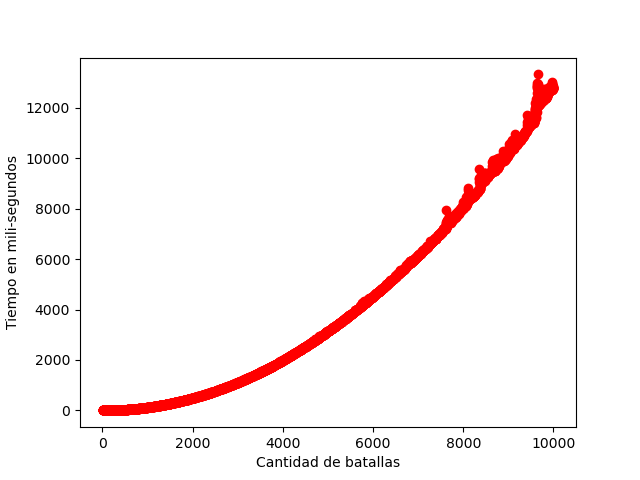
\includegraphics[scale=0.69]{graficoComplejidadVintage.png}

Podemos ver que el gráfico tiene una forma cuasi parabólica, lo cual refleja el comportamiento cuadrático del algoritmo.

Además, podemos ver el rápido crecimiento que toman los valores. Por ejemplo, 1000 minutos de combate tardan alrededor de 160 mili-segundos y con $n = 2000$ el algoritmo tarda más de 600 mili-segundos. Vemos que al duplicar el tamaño de la entrada, el tiempo que tarda no se duplica, sino que se cuadruplica.

La segunda corrida de tests tuvo resultados análogos:

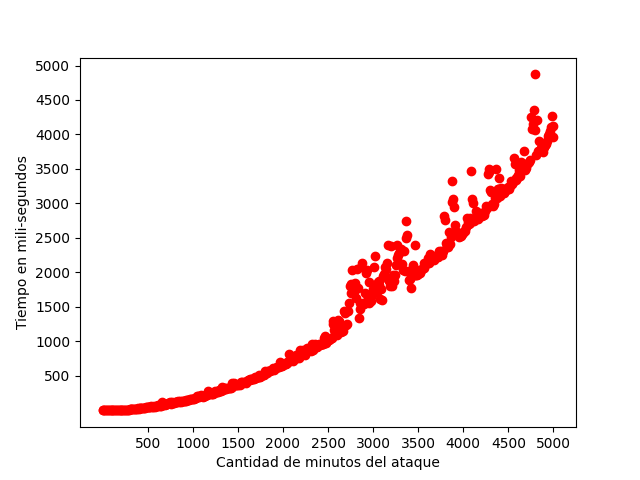
\includegraphics[scale=0.69]{graficoComplejidad.png}


Este también tiene una forma cuasi parabólica y también hay un rápido crecimiento del tiempo que le lleva al  algoritmo cuando aumentamos los valores. Con, 1000 minutos de combate tardan alrededor de 160 mili-segundos y con $n = 2000$ el algoritmo tarda más de 600 mili-segundos. Se repite el patrón que al duplicar el tamaño de la entrada, el tiempo que tarda no se duplica, sino que se cuadruplica.

Con esto concluimos que, a medida que aumenta el tamaño de entrada $n$ (cantidad de minutos), el tiempo de ejecución del algoritmo crece a un ritmo cuadrático. Esto coincide con el análisis de complejidad previamente presentado, indicando un costo proporcional a $n^2$.

\end{document}